\section{Itération n°3}

\subsection{Objectif de l'itération}

Dans cette nouvelle itération, nous allons devoir modifier notre code afin que ce dernier puisse générer du bruit et gérer les problèmes au niveau du bruit et de sa puissance. Nous allons devoir coder une nouvelle classe afin qu'elle émette un bruit gaussien. Par ailleurs, nous devrons mettre en place un code nous permettant d'échantiller les signaux bruités reçu afin qu'ils correspondent aux signaux émis.

Ci-dessous le schéma correspondant à l'itération n°3.

\begin{figure}[H]
\centering
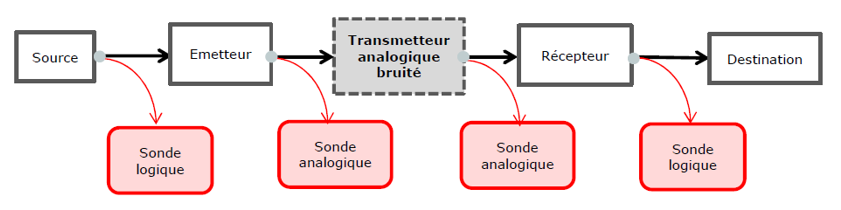
\includegraphics[width=1\textwidth]{image 16.png}
\caption{\label{fig:image16}Schéma de l'itération n°3.}
\end{figure}

Ci-dessous le schéma correspondant à l'ajout de bruit pour cette itération

\begin{figure}[H]
\centering
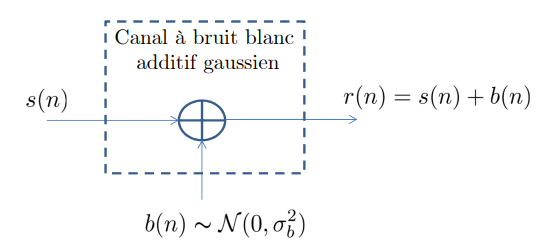
\includegraphics[width=0.8\textwidth]{image 17.png}
\caption{\label{fig:image17}Schéma d'ajout de bruit itération n°3.}
\end{figure}

Dans cette partie on nous demande également un graphique représentant le taux d'erreur binaire (TEB) en fonction du rapport signal sur bruit (SNR) par bit. Nous devons donc faire des modifications dans notre code afin de calculer le SNR et de modéliser la courbe.

\subsection{Organisation}

Pour nous permettre de répondre aux demandes de l'itération (mise en place de l'ajout d'un bruit blanc gaussien), nous allons devoir créer de nouveaux éléments par rapport au code de l'itération précédente. Ces modifications devront nous aider à lancer le programme tout en prenant en compte le bruit qui pourrait se trouver dans un canal de transmission. Nous ne devrions pas avoir d'erreurs sur notre code cependant nous devrions pouvoir observer l'ajout de bruit que nous avons effectué sur nos graphiques lors de la modélisation de notre signal transmis à la destination. Afin de vérifier le bon fonctionnement de notre code nous nous appuirons sur ces graphiques mais également sur les calculs du TEB, du SNR ainsi que sur la courbe TEB vs SNR.
En vue des modifications à effectuer, nous avons développé le diagramme de Gant que nous avions utilisé lors de la première itération afin d'affecter à chacuns des tâches pour permettre de pouvoir livrer l'itération à l'heure. Vous trouverez ci-dessous le diagramme de Gant pour cette troisième itération :

\begin{figure}[H]
\centering
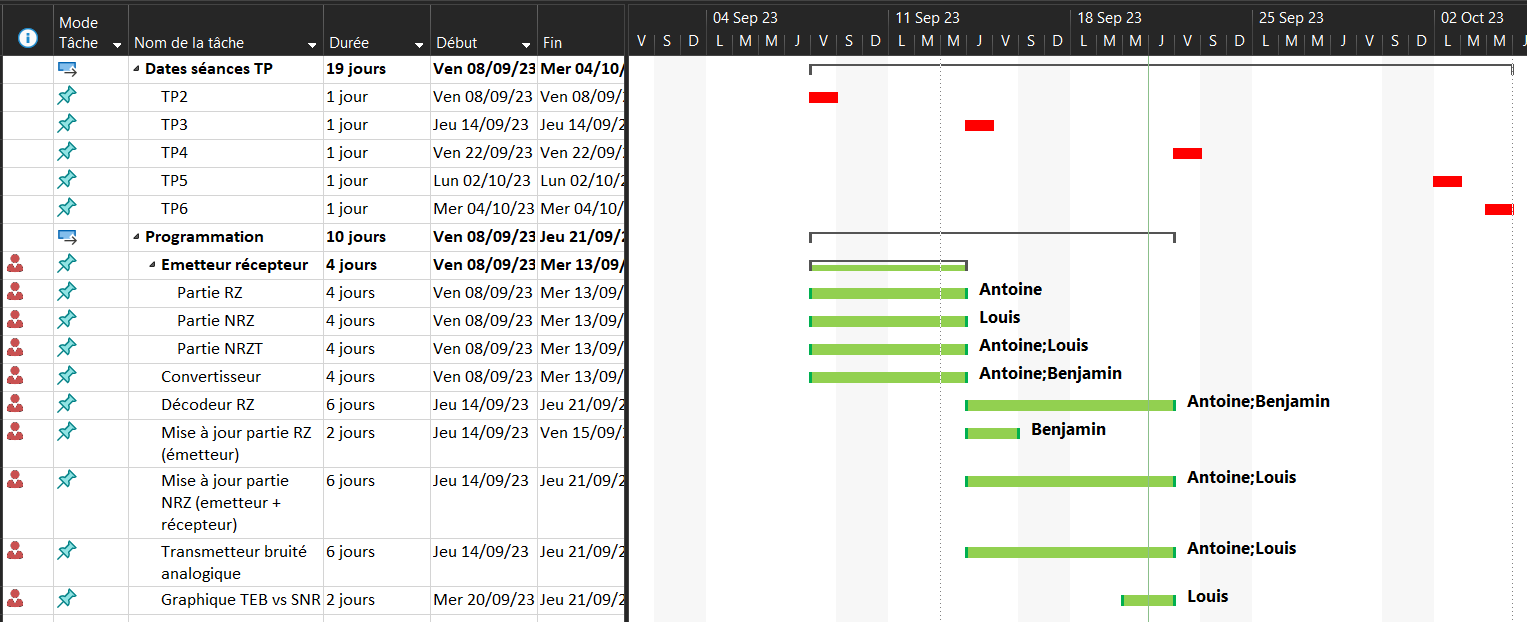
\includegraphics[width=1\textwidth]{image 18.png}
\caption{\label{fig:image18}Diagramme de Gant itération 3 (1/2).}
\end{figure}
\begin{figure}[H]
\centering
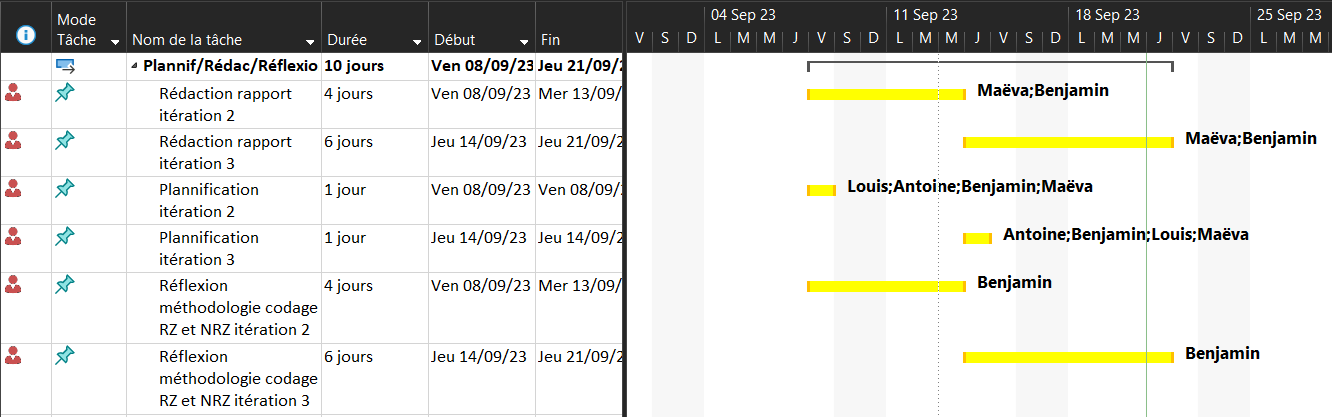
\includegraphics[width=1\textwidth]{image 20.png}
\caption{\label{fig:image20}Diagramme de Gant itération 3 (2/2).}
\end{figure}

Pour le développement de notre code nous avons utilisé l'application de bureau Intellij Idea, comme évoqué pour la seconde itération. Nous utiliserons cette application tout au long du TP. Nous avons également utilisé GitLab nous permettant de stocker le projet. Nous l'utiliserons également tout du long du TP.

\subsection{Procédures de développement}

Afin de répondre aux exigences de l'itération nous avons créé une nouvelle classe de type de composant transmetteur qui se nomme TransmetteurBruiteAnalogique. Le transmetteur est un élément clé dans une chaîne de transmission. Dans notre cas, ce dernier est analogique et nous permet donc de transmettre un signal analogique à partir d'informations numériques faites à base de 0 et de 1.

Dans cette itération, nous nous intéressons à la modulation du bruit et de son ajout au code et au signal final. Afin de modéliser ce bruit nous avons besoin de formules mathématiques que nous pouvons retrouver par raisonnement.

\subsubsection{Modélisation du bruit}
Pour la création de notre bruit nous utilisons la formule suivante :
$b(n) = \sigma_b\sqrt{-2*ln(1-a_1 (n))}cos(2\pi*a_2 (n))$ avec $a_1 (n) ~ \mathcal{U}[0,1[$ (loi uniforme) et $a_2 (n) ~ \mathcal{U}[0,1[$

Pour l'utiliser, il faut calculer la variance.
$\sigma = \sqrt{\frac{P_s*N}{2*10^{\frac{SNR}{10}}}}$
On remarque que notre bruit est généré en fonction de notre SNR.

Il nous reste plus qu'à injecter dans notre signal analogique le bruit généré précédemment. Ainsi, nous arrivons à simuler un signal bruité comme similaire dans la vraie vie à son arrivée dans le récepteur. Grâce à celui-ci, nous allons pouvoir tester la performance de nos codages de ligne.

\subsection{Performances}

Pour tester la perormance de ce système, on va générer deux fonctions permettant de vérifier deux paramètres différents.

\subsubsection{Graphe gaussien du bruit}

Lors de cette itération, nous avons utilisé la formule de Rice pour générer le bruit que l'on va additionner dans notre canal. Pour vérifier que notre bruit est bien blanc et gaussien, nous allons  dessiner un graphique qui va avoir comme données la puissance de bruit par rapport au nombre d'occurrence (voir le graphique ci-dessous).

\begin{figure}[H]
\centering
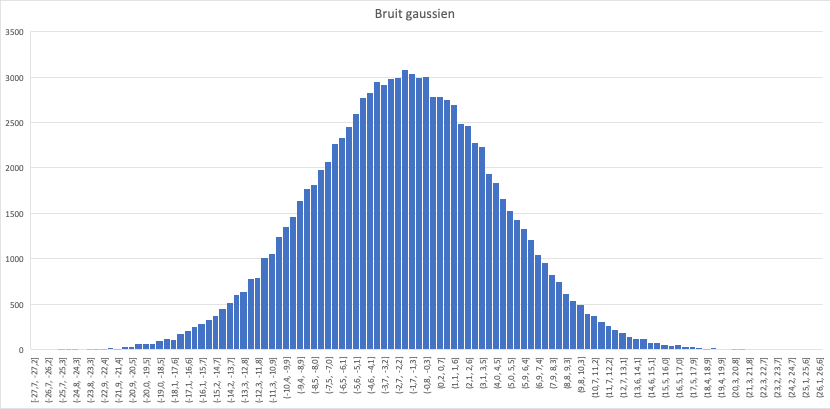
\includegraphics[width=1\textwidth]{img/gaussienne.png}
\caption{\label{fig:gaussienne}Gaussienne}
\end{figure}

\subsubsection{Test de la performance des codages de canal}

La deuxième série de valeur à générer permet de savoir à quelle SNR notre codage de ligne est considéré comme fiable.
Pour ce faire, on va tracer un graphique représentant le TEB en fonction du $\frac{RSB}{bit}$.

\begin{figure}[H]
\centering
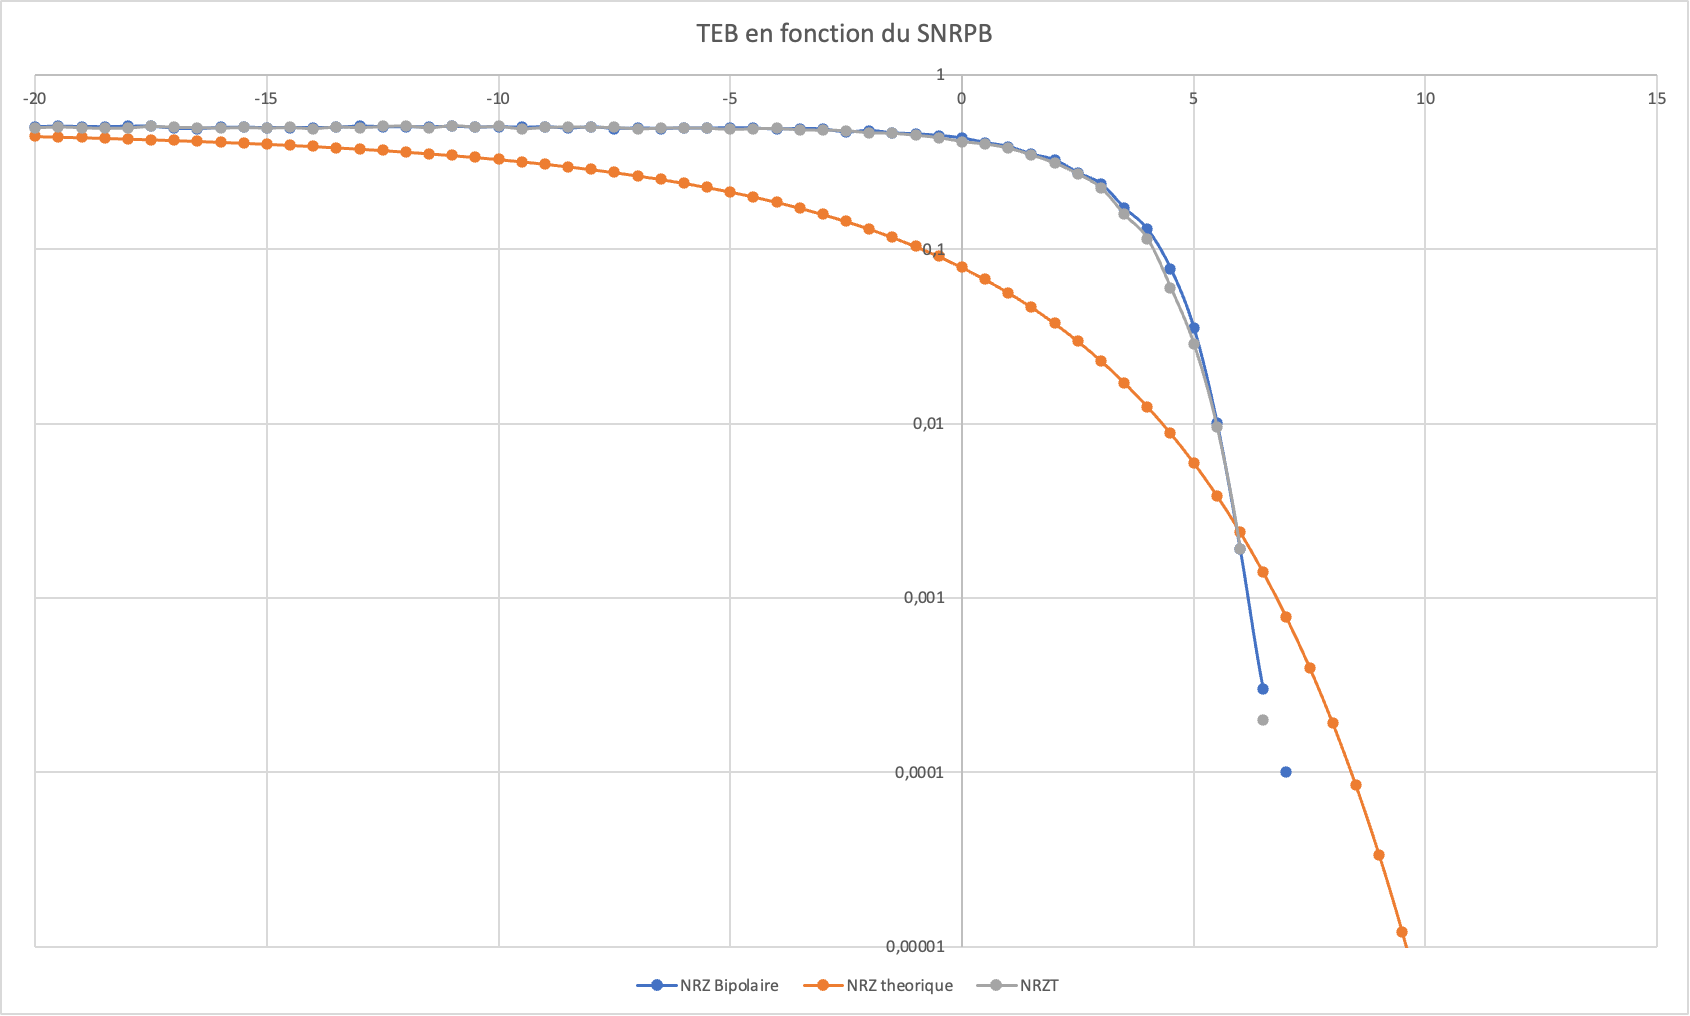
\includegraphics[width=0.9\textwidth]{img/tebvssnrpb.png}
\caption{\label{fig:TEBenFonctionDesSNR}Graphique du TEB en fonction du SNRPB.}
\end{figure}

\textcolor{red}{Après correction de notre calcul du bruit blanc gaussien, nous trouvons désormais des valeurs plus proche de la réalité. La courbe orange représente le TEB théorique du NRZ. Nous constatons que notre méthode de réception peut être améliorée mais quelle semble parfaitement gérer un signal bruité avec un snrpb de 5 et au delà}

On remarque que le signal NRZ est le signal qui a le plus robuste au bruit car son TEB est le premier à descendre  en asymptote pour un SNR/bit de -7. Il est suivi du NRZT et du RZ. La performance du codage NRZ est peut-être du au fait qu'il est défini sur un intervalle Amax et Amin plus important que le NRZT/RZ

\subsection{Conclusion}

Cette troisième étape nous a permis de comprendre plus en détail les problèmes liés au bruit dans les canaux de transmission. Nous avons pu manipuler les équations liés au bruit notamment le SNR (rapport signal sur bruit) afin de trouver la puissance du bruit et le sigma du bruit afin de trouver la génération du bruit gaussien. Cela nous a donc permis de manipuler le bruit au sein de notre code afin de modéliser un canal de transmission bruité tout en nous permettant de retrouver le signal de départ.
Nous avons également eu des problèmes de gestion du temps. Suite aux complications que nous avions eu à l'itération précédente, nous avions dû corriger nos erreurs et donc nous avions eu moins de temps pour coder cette troisième itération. De ça, nous n'avons pas eu assez de temps pour modéliser nos tests.
Lors de la prochaine étape, nous allons devoir pousser un peu plus loin le bruit. Nous allons devoir modéliser et gérer des bruit "réels" tel que les bruits de trajets-multiples, de dispersion chromatique et de bruit électrique.